\chapter{Bases Mathématiques du calcul fractionnaires}
\label{chap:Préliminaires}
\pagestyle{fancy}
Avant d'aborder les fonctions essentielles, il est nécessaire de réviser les théorèmes fondamentaux qui joueront un rôle important dans le développement futurs de notre étude
\section{Prérequis du Calcul Ordinaire}
\subsection*{Théorème fondamental de l'analyse}
Ce théorème établit un lien profond entre les deux opérations principales du calcul, la dérivation et l'intégration. Il nous dit que l'intégrale d'une fonction sur un intervalle peut être obtenue en trouvant une fonction primitive et en la évaluant aux extrémités de cet intervalle. Cette relation fondamentale entre l'intégrale et la dérivée est le pilier du calcul différentiel et intégral.
    \begin{equation}\label{FTC}
        \frac{d}{dt}\int_a^t f(t) = f(t) \hspace{1cm} \forall t\in[a,b]
    \end{equation}
\subsection*{Changement d'ordre d'intégration}
Le changement d'ordre d'intégration est une astuce que nous utiliserons par exemple lors du calcul de l'intégral fractionnaire de la fonction de puissance. Nous soulignons que ce processus n'impose aucune nouvelle condition pour la fonction intégrée, il s'agit simplement d'une vision différente de la zone sur laquelle nous intégrons.

Selon \cite{FDE&applications} Il existe des versions plus générales connues (par exemple le théorème de Fubini), mais pour nous, le cas des zones triangulaires est suffisant. La formule suivante \ref{C_O_I} est valable pour toutes les fonctions $f (t, \tau, \xi)$ intégrables par rapport à $\tau$ et $\xi$.

\begin{equation}\label{C_O_I}
    \int_{a}^{t} \int_{a}^{\tau} f(t, \tau, \xi) d\xi d\tau = \int_{a}^{t} \int_{\xi}^{t} f(t, \tau, \xi) d\tau d\xi
\end{equation}

%plot
{
\centering
\begin{minipage}[t]{.5\textwidth}
    \begin{flushleft}
        \resizebox{\textwidth}{!}{
        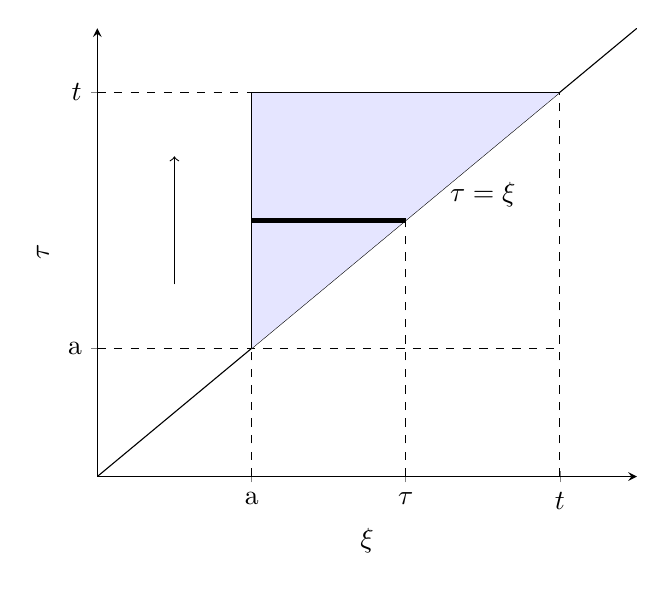
\begin{tikzpicture}
    \begin{axis}[ 
        xlabel=$\xi$, 
        ylabel=$\tau$, 
        xlabel near ticks, % move x label closer to the ticks
        ylabel near ticks, % move y label closer to the ticks
        axis lines=left, 
        xtick={1, 2, 3}, % specify the x-ticks
        xticklabels={a, $\tau$, $t$}, 
        ytick={1, 3}, % specify the y-ticks
        yticklabels={a, $t$},
        domain=0:4, % specify the domain
        xmin=0, xmax=3.5, % specify the x limits
        ymin=0, ymax=3.5, % specify the y limits
        samples=100
    ]
        \addplot[color=black]{x}; % plot the line x=y
        \draw[dashed] (axis cs:1,0) -- (axis cs:1,1); % draw the vertical line at x=a
        \draw[dashed] (axis cs:2,0) -- (axis cs:2,2); % draw the vertical line at x=tau
        \draw[dashed] (axis cs:3,0) -- (axis cs:3,3); % draw the vertical line at x=t
        \draw[dashed] (axis cs:0,3) -- (axis cs:3,3); % draw the horizontal line at y=t
        \draw[dashed] (axis cs:0,1) -- (axis cs:3,1); % draw the horizontal line at y=a

        % fill the area first
        \addplot[fill=blue!10] coordinates {(1,1) (1,3) (3,3)};

        % then add the line you want to appear over the filled area
        \addplot[ultra thick, domain=1:2]{2};

        % add the label over the filled area
        \node at (axis cs:2.5,2.2) {$\tau=\xi$};

        % draw an arrow pointing upwards from the middle of the shape
        \draw[->] (axis cs:0.5,1.5) -- (axis cs:0.5,2.5);
    \end{axis}
\end{tikzpicture}
}%
    \end{flushleft}
\end{minipage}%
\begin{minipage}[t]{.5\textwidth}
    \begin{flushright}
        \resizebox{\textwidth}{!}{
        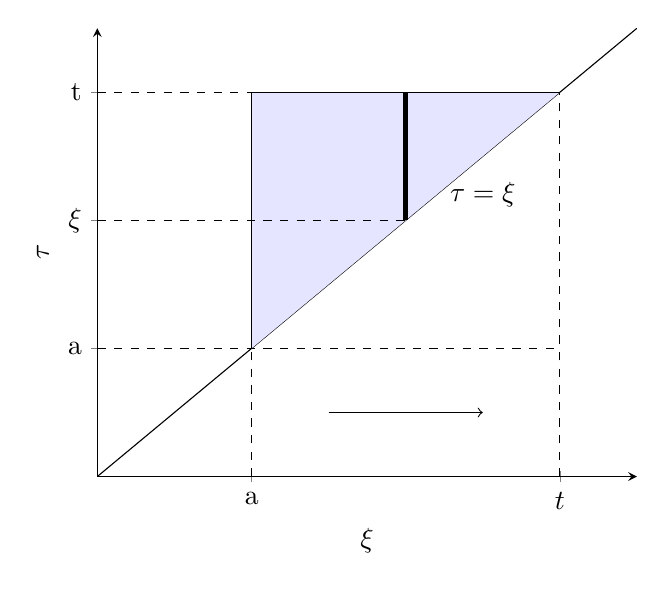
\begin{tikzpicture}
    \begin{axis}[ 
        xlabel=$\xi$, 
        ylabel=$\tau$, 
        xlabel near ticks, % move x label closer to the ticks
        ylabel near ticks, % move y label closer to the ticks
        axis lines=left, 
        xtick={1, 3}, % specify the x-ticks
        xticklabels={a, $t$}, 
        ytick={1, 2, 3}, % specify the y-ticks
        yticklabels={a, $\xi$, t},
        domain=0:4, % specify the domain
        xmin=0, xmax=3.5, % specify the x limits
        ymin=0, ymax=3.5, % specify the y limits
        samples=100
    ]
    
        \addplot[color=black]{x}; % plot the line x=y
        
        % fill the area first
        \addplot[fill=blue!10] coordinates {(1,1) (1,3) (3,3)};
        
        \draw[dashed] (axis cs:1,0) -- (axis cs:1,1); % draw the vertical line at x=a
        \draw[dashed] (axis cs:3,0) -- (axis cs:3,3); % draw the vertical line at x=tau
        \draw[dashed] (axis cs:0,1) -- (axis cs:3,1); % draw the vertical line at x=t
        \draw[dashed] (axis cs:0,2) -- (axis cs:2,2); % draw the horizontal line at y=t
        \draw[dashed] (axis cs:0,3) -- (axis cs:3,3); % draw the horizontal line at y=a

        % then add the line you want to appear over the filled area
        %\addplot[ultra thick, domain=1:2]{2};
        \draw[ultra thick] (axis cs:2,2) -- (axis cs:2,3);
        % add the label over the filled area
        \node at (axis cs:2.5,2.2) {$\tau=\xi$};

        % draw an arrow pointing upwards from the middle of the shape
        \draw[->] (axis cs:1.5,0.5) -- (axis cs:2.5,0.5);
    \end{axis}
\end{tikzpicture}
        }%
    \end{flushright}
\end{minipage}
\captionof{figure}{Illustration géométrique - Changement d'ordre d'intégration}
}
\subsection*{Dérivé d'un Intégrale paramétrique}
Comme nous le verrons plus tard, les intégrales et dérivées d'ordre non entiers sont généralement présentées sous la forme d'une intégrale dépendant d'un paramètre qui est égal à la limite supérieure d'intégration. Il est donc très important de connaître la règle pour la dérivée par rapport à ce paramètre.

Il peut être prouvé que la formule suivante est valable lorsque la fonction intégrée $g(t, \tau)$ est intégrable par rapport à la seconde variable, sa dérivée $ \frac{\partial}{\partial t} g(t, \tau) $ est continue et $g(t, \tau)$ est définie en tous points $(t, t)$ .
\begin{equation*}
    \frac{d}{dt}\int_{a}^{t} g(t,\tau) d\tau = g(t,t) + \int_{a}^{t} \frac{\partial}{\partial t} g(t,\tau) d\tau
\end{equation*}

Dans le calcul fractionnaire, nous travaillons souvent avec des fonctions du type $g(t, \tau) = (t-\tau)^{r} f(\tau) $ pour un certain $r \geq 0$, examinons donc le résultat dans une telle situation. Le cas $r = 0$ est assez trivial (nous obtenons simplement $f(t)$), sinon nous obtenons la formule \ref{Derive_I_para} ci-dessous puisque dans ce cas $g(t, t) = 0$ pour tout $t$

\begin{equation} \label{Derive_I_para}
        \frac{d}{dt}\int_{a}^{t} (t-\tau)^r f(\tau) d\tau = r \int_{a}^{t} (t-\tau)^{r-1} f(\tau) d\tau
\end{equation}
\section{Fonction Gamma}
La naissance de la fonction Gamma résulte de la volonté de prolonger la fonction factorielle à l'ensemble des nombres non-entier. Grâce à Euler \cite{LEI}, Gauss et d'autre mathématicien, cette extension naturelle a offert l'opportunité de traiter différent problèmes mathématiques et physiques.
Dans l'analyse fractionnaire, la puissance de la fonction Gamma réside dans la notion de dérivée et d'intégrale d'ordres non entiers \cite{Frac_Cal_WolframeAlpha}.
De plus, elle fournit le cadre nécessaire pour définir d'autres fonctions importantes qui sont essentielles dans l'étude et la résolution des EDF.\\
Nous limiterons dans ce rapport à la définition de cette fonction sur l'ensemble des réels $\mathbb{R}^+$.
\begin{definition} On désigne par $\Gamma (x)$ la fonction définie dans l'intervalle $]0,+\infty[$, par l'intégrale généralisée suivant
    \begin{equation}
        \Gamma(x)=\int_{0}^{\infty} e^{-t} t^{x-1}dt.
    \end{equation}
    (seconde intégrale eulérienne)
\end{definition} 
La fonction $\Gamma$ est bien définie, soient
$f \colon \mathbb{R} \times \mathbb{R^{*+}} \to \mathbb{R}\times \mathbb{R}, (x,t)\mapsto e^{-t} t^{x-1}$ et pour tout $x \in \mathbb{R}$, $f_x \colon \mathbb{R^{*+}} \to \mathbb{R},
\quad t \mapsto f(x,t)$
quel que soit $x\in \mathbb{R}$, $f_x$ est définie, continue, positive sur $]0,+\infty[$ donc $\Gamma(x)$ est définie lorsque $f_x$ est intégrable sur $]0,+\infty[$.\\
\begin{itemize}
    \item En $0$, $f_x(t) \underset{t \to 0}{\sim}  t^{x-1}$ donc $f_x$ est intégrable sur $]0,1[$ si et seulement $x>0$.
    \item En $+\infty$, $f_x(t) = o(\frac{1}{t^2})$ donc $f_x$ est intégrable sur $[1, +\infty].$ $ \lim_{x\to +\infty}t^2 f_x(t) = \lim_{x\to +\infty} t^{x+1}e^{-t} = \lim_{x \to +\infty} e^{-t\left[1+(x-1)\frac{ln(t)}{t}\right]} = 0 $ donc il résulte du critère de Riemann que la fonction $f_x$ est intégrable au voisinage de $+\infty$.
\end{itemize}
Finalement, $\Gamma(x) $ est définie si et seulement si $x \in ]0,+\infty[$
\begin{figure}[H]
    \centering
    \includegraphics[scale = 0.7]{IMAGES/gamma_func.png}
    \caption{La fonction Gamma}
    \label{fig:gamma_fact}
\end{figure}
\begin{exemple}
    \begin{enumerate}
        \item $\Gamma(1) = 1$
        \item Pour $x=\frac{1}{2}$ on a 
        \begin{equation*}
            \Gamma(\frac{1}{2}) = \int_{0}^{+\infty} t^{\frac{1}{2}-1} e^{-t} dt = \int_{0}^{+\infty} t^{\frac{-1}{2} e^{-t} dt}.
        \end{equation*}
        On pose $ t = u ^ 2 $, alors $dt = 2udu$. On obtient
        \begin{equation*}
            \Gamma(\frac{1}{2}) = \int_{0}^{+\infty} t^{\frac{-1}{2}} e^{-1}dt = 2\int_{0}^{+\infty} e^{-u^2} du.
        \end{equation*}
        avec $r \in [0, +\infty[$  et $ 0  \leq \theta \leq \frac{\pi}{2}$. Alors
        \begin{align*}
            \left[\int_{0}^{+\infty} e^{{-u^2}} du\right]^2 &= \int_{0}^{+\infty} e^{-u^2} du\int_{0}^{+\infty} e^{-v^2} dv
            \\
            &= \int_{0}^{+\infty}\int_0^{+\infty} e^{-(u^2+v^2)} dudv\\ 
            &= \int_{0}^{\frac{\pi}{2}}d\theta \int_{0}^{+\infty} r e^{-r^2} dr\\
            &= \frac{\pi}{2}\left[ -\frac{1}{2} e^{-r^2}\right]_0^{+\infty} = \frac{\pi}{2}
        \end{align*}
        et par suite 
        \begin{equation*}
            \Gamma(\frac{1}{2})=\int_0^{+\infty} t^{-\frac{1}{2}} e^{-t} dt = 2\int_0^{+\infty} e^{-u^2} du = \sqrt{\pi}
        \end{equation*}
    \end{enumerate}
\end{exemple}
L'intégral d'Euler ne converge pas pour les 
$\Re(x)<0$. Mais on peut prolonger $\Gamma(x)$ (figure \ref{fig:gamma_fact}), puisque la fonction qu'elle définie dans la demi-plan complexe positive a une continuation analytique unique dans la moitié négatif du plan, on peut calculer la fonction Gamma pour les arguments positifs (\ref{gamma_tout_entiers}) en utilisant l'intégrale d'Euler, puis étendre les résultats pour inclure les nombres négatifs en utilisons la formule de récurrence de la fonction Gamma (\ref{gamma_n}).
\begin{proposition}
    Soient $n\in \mathbb{N}$. On a les identités suivantes:
        \begin{enumerate}
            \item $\Gamma(x+1) = x\Gamma(x)$, pour tout $x > 0$\label{gamma_n}
            \item $\Gamma(x+n) = x(x+1) ... (x+n-1)\Gamma(x)$, \label{gamma_tout_entiers} pour tout $x\in \mathbb{R \textbackslash Z^-}$ tel que $ -n < \Re(x) \leq -n+1 $.
        \end{enumerate}
    
\end{proposition}
\begin{proof}
    \begin{enumerate}
        \item Soit $x>0$. Nous procédons par l'usage d'une intégration par parties.\\
        \begin{align*}
            \Gamma(x+1) &= \int_{0}^{\infty} t^x e^{-t} dt \\
            &= \left[ -t^x e^{-t} \right]_0^{+\infty} + \int_{0}^{+\infty} xt^{x-1} e^{-t} dt\\ 
            &= \lim_{t \to +\infty} (-t^x e^{-x}) + x\int_{0}^{+\infty} t^{x-1}e^{-t} dt.
        \end{align*}
        Et clairement $\lim_{t \to +\infty} (t^x e^{-t}) = 0$. Donc, on en déduit par la définition de $\Gamma(x)$ que $\Gamma(x+1) = x\Gamma(x)$. \label{gamma_n}
        \item C'est une conséquence immédiate de l'identité (\ref{gamma_n}) et le principe de récurrence.
    \end{enumerate}
\end{proof}
\begin{remarque}
    Si on prend $x=1$ dans la propriété (\ref{gamma_tout_entiers}), on obtient
    \begin{equation*}
        \Gamma(n+1)=n! \hspace{1cm} \forall n \in \mathbb{N}.
    \end{equation*}
    Et cela démontre ce que nous avons dit précédemment, que le fonction gamma est la généralisation de la notion de la factorielle pour $x > 0$.
\end{remarque}
\begin{figure}[H]
    \centering
    \includegraphics[scale = 0.7]{IMAGES/gamma.png}
    \caption{La relation géométrique entre la Fonction Gamma dans le domaine réel et la factorielle}
    \label{fig:gamma_fact}
\end{figure}

\begin{theoreme}
    La fonction $\Gamma$ possède les propriétés suivantes :
    \begin{enumerate}
        \item $\Gamma$ est continue sur $]0,+\infty[$.
        \item $\Gamma$ est de classe $C^{\infty}$ sur $]0, \infty[$ avec\\
        \begin{equation*}
            \Gamma^{(k)}(x) = \int_{0}^{\infty} t^{x-1}(\ln t)^k e^{-t} dt \hspace{1cm} \forall x >0, \forall k\in\mathbb{N}
        \end{equation*}
        \item $\Gamma$ est convexe.
    \end{enumerate}
\end{theoreme}
\begin{proof}
    \begin{enumerate}
        \item $f$ est continue sur $(\mathbb{R^{*+}})^2$, et pour tout $x\in \mathbb{R^{*+}}$, $f_x$ est intégrable sur $]0,+\infty[$. \\
        Montrons alors que $f$ satisfait à l'hypothèse de domination pour $x$ décrivons $[a,b]$, $a<b$, intervalle compact quelconque inclus dans $\mathbb{R^{*+}}$.\\ 
        Pour $0<t\leq 1$, $x \to t^{x-1}$ est décroissante donc pour $x\in [a,b]$, on a $0<f(x,t)\leq t^{a-1}$\\
        Pour $t\geq1$, $x\to t^{x-1}$ est croissante, et alors $x\in [a,b]$ donne $0<f(x,t)\leq e^{-t} t^{b-1}$.\\
        Soit alors $\phi:]0,+\infty[ \to \mathbb{R}$, $t \to \phi(t)$ ..\\
        $\phi$ est positive, continue par morceaux et intégrable sur$]0,+\infty[$ et 
        \begin{equation*}
            \forall(x,t)\in [a,b] \times ]0,+\infty[, \hspace{1cm} 0<f(x,t)\leq \phi(t)
        \end{equation*}
        Ainsi $\Gamma$ est continue sur $]0,+\infty[$ d'après le théorème de continuité sous le signe somme.
        \item Pour tout $k \in \mathbb{N^*}$, $f$ est de classe $C^k$ sur $(\mathbb{R^{*+}})^2$ avec \\
        \begin{equation*}
            \forall(x,t)\in(\mathbb{R^{*+}})^2, \hspace{1cm} \frac{\partial ^k f}{\partial x^k}(x,t)=(\ln t)^k e^{-t} t^{x-1}
        \end{equation*}  
        Considérons de nouveau un intervalle compact $[a,b]\subset \mathbb{R^{*+}}$ et soit $\psi _k : ]0,+\infty[ \mapsto \mathbb{R}$ telle que
        \begin{equation*}
            \forall t\in ]0,+\infty[, \hspace{1cm} \psi_k (t) = |\ln t|^k \phi(t)
        \end{equation*}
        Au voisinage de 0, on a $\psi_k (t) = o\left(\frac{1}{t^{1-\frac{a}{2}}} \right)$ et en $+\infty$, on a encore $\psi _k (t) = o\left(\frac{1}{t^2}\right)$ donc $\psi_k$ est positive, continue par morceaux et intégrale sur $]0,+\infty[$.\\
        Par construction, on a 
        \begin{equation*}
            \forall(x,t)\in[a,b]\times]0,+\infty[, \hspace{1cm} \left| \frac{\partial ^k f}{\partial x^k} (x,t) \right| \leq \psi _k(t)
        \end{equation*}
        Montrons par récurrence que pour tout $k\in\mathbb{N^*}$, $\Gamma$ est de classe $C^k$ sur $\mathbb{R^{+*}}$ avec:
        \begin{equation*}
            \mathcal{P} (k): \hspace{1cm} \forall x\in\mathbb{R^{*+}}, \Gamma^{(k)} (x) = \int_0^{+\infty} (\ln t)^k e^{-t} t^{x-1} dt
        \end{equation*}
        La classe $C^1$ de $f$ sur $(\mathbb{R^{*+}})^2$ et l'étude de la définition de $\Gamma$ assurent les premières hypothèses du théorème de dérivation sous le signe somme et les fonctions $\psi_1$ donnent l'hypothèse de domination sur tout segment $[a,b]\subset \mathbb{R^{*+}}$.(Il y a une fonction $\psi_1$ pour chaque segment $[a,b] \subset\mathbb{R^{*+}}$).\\
        Ainsi, par application du théorème, $\Gamma$ est de classe $C^1$ sur $\mathbb{R^{*+}}$ avec :
        \begin{equation*}
            \forall x\in\mathbb{R^{*+}}, \hspace{1cm} \Gamma'(x)=\int_0^{+\infty}(\ln t)e^{-t} t^{x-1}dt
        \end{equation*}
        C'est-à-dire la propriété $\mathcal{P}(1)$ est vraie.\\
        Montrons maintenant que si $\mathcal{P}(k)$ est vraie, alors $\Gamma^{(k)}$ est de classe $C^1$ sur $\mathbb{R^{*+}}$.\\
        La classe $C^{k+1}$ de $f$ sur $(\mathbb{R}^{*+})$ donne la classe $C^1$ sur $(\mathbb{R}^{*+})^2$ de $\frac{\partial ^k k}{\partial x^k}$ et $\Gamma ^{(k)}$ étant définie pour tout $x\in\mathbb{R}^{*+}$, les premières hypothèses du théorème de dérivation sous le signe somme sont vérifiées pour la fonction $g=\frac{\partial ^k f}{\partial x^k}$. D'autre part, les fonctions $\psi _{k+1}$ montrent que $\frac{\partial g}{\partial x} = \frac{\partial ^{k+1} f}{\partial x^ {k+1}}$ satisfait à l'hypothèse de domination sur tout segment $[a,b]\subset \mathbb{R}^{*+}$. On en déduit que $\Gamma ^{(k)}$ est de classe $C^1$ sur $\mathbb{R}^{*+}$, c'est-à-dire que $\Gamma$ est de classe $C^{k+1}$ avec
        \begin{equation*}
            \forall x\in \mathbb{R}^{*+}, \hspace{1cm} \Gamma^{(k+1)}(x)=\int_0^{+\infty} (\ln t)^{k+1} e^{-t} t^{x-1} dt 
        \end{equation*}
        La propriété $\mathcal{P}(k)$ est donc héréditaire, ce qui achève d'établir que $\Gamma$ est de classe $C^k$ sur $\mathbb{R}^{*+}$ pour tout $k\in \mathbb{N}^*$, donc que $\Gamma$ est de classe $C^{+\infty}$.
        \item $\Gamma ''(x) = \int_0^{+\infty} (\ln t)^2 e^{-t}t^{x-1}dt $, $\Gamma ''$ est strictement positive sur $\mathbb{R}^{*+} $ donc $\Gamma$ est convexe.
    \end{enumerate}
\end{proof}
\section{Fonction Bêta}
\begin{definition}
On désigne par $\beta(x,y)$ la fonction définie pour $x>0$ et $y>0$
par l’intégrale suivant:
    \begin{equation}
        \beta(x,y) = \int_{0}^{1} t^{x-1}(1-t)^{y-1} dt
    \end{equation}
    (première intégrale eulérienne)
\end{definition}

La fonction $\beta$ est bien définie sur $]0,+\infty[\times]0,+\infty[$.\\
Soient $(x,y)\in]0,\infty[\times]0,+\infty[:$\\
\begin{itemize}
    \item $t^{x-1}(1-t)^{y-1} \underset{t \to 0^+}{\sim} t^{x-1}$, et $0\leq \int_0^{\frac{1}{2}} t^{x-1}dt < +\infty $  car  $x>0$ donc $1-x<1$.
    \item $t^{x-1}(1-t)^{y-1}\underset{t \to{1}}{\sim}(1-t)^{y-1}$, et $0\leq\int_{\frac{1}{2}}^1 (1-t)^{y-1} dt <+\infty$ car $y>0$ donc $1-y<1$. 
\end{itemize}
Par suite $\int_0^1 t^{x-1}(1-t)^{y-1}dt$ est convergente.
\begin{figure}[H]
    \centering
    \includegraphics[scale = 0.7]{IMAGES/betaFunc.png}
    \caption{La fonction Bêta}
\end{figure}
\begin{theoreme}
    La fonction bêta est symétrique, on a
    \begin{equation}
        \beta(x,y)=\beta(y,x)
    \end{equation}
\end{theoreme}
\begin{proof}
    On considère le changement de variable $u=1-t$. Alors pour tout $x,y>0$, on a 
    \begin{equation*}
        \beta(x,y) = \int_0^1 t^{x-1}(1-t)^{y-1}dt=\int_0^1 (1-u)^{x-1} u^{y-1}du =\beta(y,x).
    \end{equation*}
\end{proof}
\begin{theoreme}
    La relation avec la fonction Gamma\\
    \begin{equation}
        \beta(x,y) = \frac{\Gamma(x)\Gamma(y)}{\Gamma(x+y)} = \frac{(x-1)!(y-1)!}{(x+y-1)!}.
    \end{equation}
\end{theoreme}
\begin{proof}
    Soit $x,y >0$, on a 
    \begin{align*}
        \Gamma(x)\Gamma(y) &= \int_0^{+\infty} e^{-t}t^{x-1}dt\int_0^{+\infty} e^{-u}u^{y-1} du\\
        &= \int_0^{+\infty}\int_0^{+\infty} e^{-(t+u)}t^{x-1}u^{y-1} dtdu \\
        &= \int_0^{+\infty}t^{x-1} dt \int_0^{\infty} e^{-(t+u)}u^{y-1}du.
    \end{align*}
    En utilisant les changements de variables $r=x+y$ et $x=rz$ avec $0\leq t\leq \infty$ et $0\leq z\leq 1$. Alors, $dx=zdr+rdz, dy=(1-z)dr-rdz$ et $dxdy=rdzdr$, donc:
    \begin{align*}
        \Gamma(x)\Gamma(y) &= \int_0^1 z^{x-1}(1-z)^{y-1}dz\int_0^{+\infty} e^{-r}r^{x+y-1}dr \\
        &= \beta(x,y)\Gamma(x+y).
    \end{align*}
    D'où 
    \begin{equation*}
        \beta(x,y)=\frac{\Gamma(x)\Gamma(y)}{\Gamma(x+y)}
    \end{equation*}
\end{proof}
\section{Fonction Mittag-Leffler}
Tout comme la fonction exponentielle $e^x$ occupe une place importante dans la théorie des équations différentielles d'ordre entier, la fonction de Mittag-Leffler, une généralisation à un seul paramètre de celle-ci, tient un rôle significatif dans le domaine des équations différentielles d'ordre fractionnaire. Définie par une série entière, la fonction de Mittag-Leffler émerge naturellement comme solution à ces équations. \cite{Mittag-Leffler}
\begin{definition}
    \begin{equation}\label{def:mittag-leffler1}
        E_{\alpha}(x) = \sum _{k=0}^{\infty} \frac{x^k}{\Gamma(\alpha k +1)}, \hspace{1cm} \alpha>0
    \end{equation}
\end{definition}
\begin{exemple}
    valeurs particulière de la fonction de Mittag-Leffler:
    \begin{enumerate}
        \item $E_0(x)=\sum_{k=0}^{\infty} \frac{x^k}{\Gamma(1)}=\sum_{k=0}^{\inf} x^k =\frac{1}{1-x}$, (somme d'une série géométrique)
        \item $E_1(x)=\sum_{k=0}^{\infty} \frac{x^k}{\Gamma(k+1)} = \sum_{k=0}^{\infty}\frac{x^k}{k!} = e^x $, (série exponentielle)
        \item $E_2(x) = \cosh(\sqrt{x})$,
        \item $E_3(x)=\frac{1}{3} \left[e^{x\frac{1}{3}} +2e^{x\frac{1}{3}} \cos(\frac{1}{2} \sqrt{3} x^{\frac{1}{3}}) \right]$,
        \item $E_4 (x) = \frac{1}{2} \left[\cos(x^{\frac{1}{4}}) + \cosh(x^{\frac{1}{4}}) \right]$.
    \end{enumerate}
\end{exemple}
\begin{figure}[H]
    \centering
    \includegraphics[scale = 0.7]{IMAGES/MittagLeffler_1001.png}
    \caption{Les fonctions de Mittag-Leffler \cite{plot:mittag-leffler}}
\end{figure}
La fonction de Mittag-Leffler à deux paramètres $E_{\alpha,\beta}$ généralisant la définition précédente \ref{def:mittag-leffler1}
\begin{definition}
définie par le développement en série suivant:
    \begin{equation}\label{def:mittag-leffler2}
        E_{\alpha, \beta}(x) = \sum _{k=0}^{\infty} \frac{x^k}{\Gamma(\alpha k +\beta)}, \hspace{1cm} \alpha>0, \hspace{0.3cm}\beta>0
    \end{equation}
\end{definition}
la série converge pour toute valeur d'argument x, c qui fait de la fonction une fonction entière.
\begin{remarque}
    Si $\beta =1$, alors $E_{\alpha, \beta}$ coïncide avec $E_{\alpha}$
    \begin{equation}
        E_{\alpha, 1}=E_{\alpha}
    \end{equation}
\end{remarque}
\begin{exemple}
    pour x proche de zéro, nous obtenons
    \begin{enumerate}
        \item $E_{1,1} (x)=\sum_{k=0}^{\infty} \frac{x^k}{\Gamma(k+1)} = \sum_{k=0}^{\infty} \frac{x^k}{k!} = e^x$,
        \item $E_1,2(x) = \sum_{k=0}^{\infty} \frac{x^k}{\Gamma(k+2)} = \sum_{k=0}^{\infty} \frac{x^k}{(k+1)!} = \frac{1}{x} \sum_{k=0}^{\infty} \frac{x^{k+1}}{(k+1)!} = \frac{e^x - 1}{x}$
    \end{enumerate}
\end{exemple}
\begin{remarque}
    Les fonctions hyperboliques $\sinh$ et $\cosh$ sont aussi des cas particuliers de la fonction de Mittag-Leffler à deux paramètres
    \begin{enumerate}
        \item $E_{2,1} (x^2) = \sum_{k=0} ^{\infty} \frac{x^{2k}}{\Gamma(2k +1)} = \sum_{k=0}^{\infty} \frac{x^{2k}}{(2k)!} = \cosh(x)$,
        \item $E_{2,2}(x^2) = \sum_{k=0}^{\infty} \frac{x^{2k}}{\Gamma(2k+2)} = \frac{1}{x}\sum_{k=0}^{\infty} \frac{x^{2k+1}}{\Gamma(2k+1)!} = \frac{\sinh(x)}{x} $.
    \end{enumerate}
\end{remarque}
\begin{theoreme}
    la fonction de Mittag-Leffler satisfait la formule de différenciation suivante:
    \begin{equation}
        \left(\frac{d}{dx} \right)^n \left[x^{\beta-1}E_{n,\beta}(\lambda x^n) \right] = x^{\beta-n-1} E_{n,\beta-n}(\lambda x^n), \hspace{1cm} (n\in \mathbb{N}, \lambda \in \mathbb{C}).
    \end{equation}
\end{theoreme}
